\chapter*{ASIPMEISTER -ADDING NEW RESOURCE -TUTORIAL}
\section*{DEFINE, TEST and Add Hardware}
\subsection{SET THE DIRECTORIES}
\begin{enumerate}
\item Login to any \emph{\textbf{i80labpcXX.ira.uka.de}} directly or using SSH or using X2Go Client. For example, login as \emph{\textbf{asip-sajjad04}} into \emph{\textbf{i80labpc02.ira.uka.de}}
\item Open shell terminal from the start menu. It should be in your default home directory. Type ``\emph{\textbf{pwd}}''
\begin{lstlisting}
sajjad@i80pc57:~:$pwd
/home/sajjad
\end{lstlisting}
\item Create a new directory for your Lab e.g. ``\emph{\textbf{SS21''}}
\begin{lstlisting}
sajjad@i80pc57:~:$mkdir SS21
sajjad@i80pc57:~:$cd SS21/
\end{lstlisting}
\item Create a directory for your ASIP project in ``\emph{\textbf{SS21''}}
\begin{lstlisting}
sajjad@i80pc57:~/SS21:$mkdir ASIPMeisterProjects
sajjad@i80pc57:~/SS21:$cd ASIPMeisterProjects/
\end{lstlisting}
\item Create a new directory for your lab session in ``\emph{\textbf{ASIPMeisterProjects''}} e.g. ``\emph{\textbf{8''}}
\begin{lstlisting}
sajjad@i80pc57:~/SS21/ ASIPMeisterProjects:$mkdir 8
sajjad@i80pc57:~/SS21/ ASIPMeisterProjects:$cd 8/
\end{lstlisting}
\end{enumerate}
\subsection{IMPLEMENT A NEW RESOURCE AND TEST}
\begin{enumerate}[resume]
\item Write a new VHDL file of the required resource, for example, \textbf{MINMAX} to calculate the minimum and maximum from given two numbers.
\begin{lstlisting}
sajjad@i80pc57:~/SS21/ ASIPMeisterProjects/8:$vim minmax.vhd
\end{lstlisting}
\begin{lstlisting}[language=vhdl,caption={"minmax.vhd"},captionpos=t]
library IEEE;
use IEEE.STD_LOGIC_1164.ALL;

use IEEE.std_logic_arith.all;
entity minmax is
Port ( clock : in std_logic; reset: in std_logic; enb: in std_logic;
din1 : in  STD_LOGIC_VECTOR (31 downto 0);
din2   : in  STD_LOGIC_VECTOR (31 downto 0);
doutMin   : out  STD_LOGIC_VECTOR (31 downto 0);
doutMax   : out STD_LOGIC_VECTOR (31 downto 0)
);
end minmax;

architecture st of minmax is
begin
process (clock, reset, enb)
begin
if (signed(din1) < signed(din2)) then
doutMin <= din1;
else
doutMin <= din2;
end if;

if (signed(din1) > signed(din2)) then
doutMax <= din1;
else
doutMax <= din2;
end if;

end process;
end st;
\end{lstlisting}
\item Write a new VHDL or Verilog testbench file to test the new resource \textbf{MINMAX}.
\begin{lstlisting}
sajjad@i80pc57:~/SS21/ ASIPMeisterProjects/8:$vim
testbench.v
\end{lstlisting}
\begin{lstlisting}[language=verilog,caption={"testbench.v"},captionpos=t]
`timescale 1ns / 1ps

module testb;

// Inputs
reg [31:0] din1;
reg [31:0] din2;
reg clock; 
reg reset; 
reg enb;

// Outputs
wire [31:0] doutMin;
wire [31:0] doutMax;

// Instantiate the Unit Under Test (UUT)
minmax uut (
.clock(clock),
.reset(reset),
.enb(enb),
.din1(din1), 
.din2(din2), 
.doutMin(doutMin), 
.doutMax(doutMax)
);

initial begin
// Initialize Inputs
reset = 1;
clock = 1;
enb = 1;
din1 = 23;
din2 = 45;

// Wait 100 ns for global reset to finish
#1000;
// Initialize Inputs
din1 = 123;
din2 = 45;       
// Add stimulus here

end

always 
begin
clock = 1'b1; 
#20; // high for 20 * timescale = 20 ns

clock = 1'b0;
#20; // low for 20 * timescale = 20 ns
end

endmodule
\end{lstlisting}	
\item Create a new ModelSim project, add above files, compile them, and simulate the hardware to verify the functionality. Once the functionality is verified you can add it to the ASIPmeister via a FHM file.
\begin{lstlisting}
/home/sajjad/SS21/ASIPMeisterProjects/8/ASIPmeister/share/fhmdb/workdb/FHM_work
sajjad@i80pc57:~/SS21/ ASIPMeisterProjects/8:$cd
ASIPmeister/share/fhmdb/workdb/FHM_work
\end{lstlisting}
\end{enumerate}
\subsection{INCORPORATE THE RESOURCE IN ASIPMEISTER}
\begin{enumerate}[resume]
\item Copy ASIPmeister Software to a new directory for example:
\begin{lstlisting}
sajjad@i80pc57:~/SS21/ASIPMeisterProjects/8:$ cp -rf /AM/ASIPmeister .
\end{lstlisting}
\item Create FHM file of the resource from ``minmax.vhd'' using the steps in the Laboratory Script Section 4.4.
\item Copy this FHM file into ``\emph{ASIPmeister/share/fhmdb/workdb/FHM\_work}''
\begin{lstlisting}
sajjad@i80pc57:~/SS21/ ASIPMeisterProjects/8:$cd
ASIPmeister/share/fhmdb/workdb/FHM_work
sajjad@i80pc57:~/SS21/ ASIPMeisterProjects/8/
ASIPmeister/share/fhmdb/workdb/FHM_work:$vim minmax.fhm
\end{lstlisting}
\begin{lstlisting}[language=vhdl,caption={"minmax.fhm"},captionpos=t]
	<?xml version="1.0" encoding="Shift_JIS" ?>
	<FHM>
	<model_name> minmax </model_name>
	
	<model>
	<design_level> behavior </design_level>
	<version> 1.0 </version>
	<author> <![CDATA[ Joe Random Hacker ]]> </author>
	<affiliation> <![CDATA[ Uni Karlsruhe ]]> </affiliation>
	<model_info> <![CDATA[ - ]]> </model_info>
	
	<parameter>
	<parameter_value key="bit_width">
	<value> 4 </value>
	<value> 8 </value>
	<value> 16 </value>
	<value> 32 </value>
	</parameter_value>
	</parameter>
	
	<function_description>
	<script>
	<![CDATA[
	#!/usr/bin/perl
	# This script generates register function definition in behavior level
	# parameter : bit_width
	
	if ($#ARGV != 0) {
		print "number of parameters is wrong.\n";
		print "usage : this_script bit_width\n";
		exit (100);
	}
	
	$bit_width    = $ARGV[0];
	$msb = $bit_width - 1;
	
	print <<FHM_DL_FOO;
	/** minmax */
	function minmax {
		input {
			bit [31:0] din1;
			bit [31:0] din2;
		}
		output {
			bit [31:0] doutMin;
			bit [31:0] doutMax;
		}
		control {
			in clock;
			in reset;
			in enb;
		}
		protocol {
			[enb == '1'] {
				valid dout;
			}
		}
	}
	FHM_DL_FOO
	
	exit (0);
	]]>
	</script>
	</function_description>
	
	<function_conv>
	<script>
	<![CDATA[
	#!/usr/bin/perl
	# This script generates register function definition in behavior level
	# parameter : bit_width
	
	if ($#ARGV != 0) {
		print "number of parameters is wrong.\n";
		print "usage : this_script bit_width\n";
		exit (100);
	}
	
	$bit_width    = $ARGV[0];
	$msb = $bit_width - 1;
	
	print <<FHM_DL_FOO;
	/** minmax */
	function minmax {
		input {
			bit [31:0] din1;
			bit [31:0] din2;
			
		}
		output {
			bit [31:0] doutMin;
			bit [31:0] doutMax;
		}
		control {
			in bit clock;
			in bit reset;
			in bit enb;
		}
		protocol {
			single_cycle_protocol {
				enb = '1';
			}
		}
	}
	FHM_DL_FOO
	
	exit (0);
	]]>
	</script>
	</function_conv>
	
	<function_port>
	<script>
	<![CDATA[
	#!/usr/bin/perl
	# This script generates register port information in behavior level
	# parameter : bit_width
	
	if ($#ARGV != 0) {
		print "number of parameters is wrong.\n";
		print "usage : this_script bit_width\n";
		exit (100);
	}
	
	$bit_width    = $ARGV[0];
	
	$msb = $bit_width-1;
	
	print <<FHM_DL_PORTS;
	clock in bit ctrl
	reset in bit ctrl
	enb in bit ctrl
	din1 in bit_vector 31 0 data
	din2 in bit_vector 31 0 data
	doutMin out bit_vector 31 0 data
	doutMax out bit_vector 31 0 data
	FHM_DL_PORTS
	
	exit (0);
	]]>
	</script>
	</function_port>
	
	<design>
	<design_lang> vhdl </design_lang>
	
	<instance>
	<script>
	<![CDATA[
	#!/usr/bin/perl
	# This script generates register instance in behavior level
	# parameter : instance_name bit_width
	
	if ($#ARGV != 1) {
		print "number of parameters is wrong.\n";
		print "usage : this_script instance_name bit_width\n";
		exit (100);
	}
	
	$instance_name = $ARGV[0];
	$bit_width     = $ARGV[1];
	
	
	$msb = $bit_width - 1;
	
	$signals = <<END_SIGNALS;
	-- Your signal declaration here
	END_SIGNALS
	
	$vhdl = <<END_VHDL;
	-- Your vhdl code here
	process (clock, reset, enb)
	begin
	if (signed(din1) < signed(din2)) then
	doutMin <= din1;
	else
	doutMin <= din2;
	end if;
	
	if (signed(din1) > signed(din2)) then
	doutMax <= din1;
	else
	doutMax <= din2;
	end if;
	end process;
	END_VHDL
	
	
	{
		print <<FHM_DL_COMMENTS;
		FHM_DL_COMMENTS
	}
	
	
	
	print <<FHM_DL_TOP_2;
	--   int_port : internal port
	--   ext_port : external port
	
	-- Comment :
	
	library IEEE;
	use IEEE.std_logic_1164.all;
	use IEEE.std_logic_arith.all;
	
	entity $instance_name is
	port (
	FHM_DL_TOP_2
	
	print <<FHM_DL_PORTS;
	clock    : in std_logic;
	reset    : in std_logic;
	enb      : in std_logic;
	din1 : in  STD_LOGIC_VECTOR (31 downto 0);
	din2   : in  STD_LOGIC_VECTOR (31 downto 0);
	doutMin   : out  STD_LOGIC_VECTOR (31 downto 0);
	doutMax   : out STD_LOGIC_VECTOR (31 downto 0)
	);
	FHM_DL_PORTS
	
	{
		print <<FHM_DL_ARCH;
		end $instance_name;
		
		architecture st of $instance_name is
		$signals
		begin
		$vhdl
		end st;
		
		FHM_DL_ARCH
	}
	
	exit (0);
	]]>
	</script>
	</instance>
	
	<entity>
	<script>
	<![CDATA[
	#!/usr/bin/perl
	# This script generates register instance in behavior level
	# parameter : instance_name bit_width
	
	if ($#ARGV != 1) {
		print "number of parameters is wrong.\n";
		print "usage : this_script instance_name bit_width\n";
		exit (100);
	}
	
	$instance_name = $ARGV[0];
	$bit_width     = $ARGV[1];
	
	
	$msb = $bit_width - 1;
	
	{
		print <<FHM_DL_TOP;
		
		entity $instance_name is
		port (
		FHM_DL_TOP
		
	}
	
	print <<FHM_DL_PORTS;
	clock    : in std_logic;
	reset    : in std_logic;
	enb      : in std_logic;
	din1 : in  STD_LOGIC_VECTOR (31 downto 0);
	din2   : in  STD_LOGIC_VECTOR (31 downto 0);
	doutMin   : out  STD_LOGIC_VECTOR (31 downto 0);
	doutMax   : out STD_LOGIC_VECTOR (31 downto 0)
	);
	FHM_DL_PORTS
	
	{
		print <<FHM_DL_BOTTOM;
		end $instance_name;
		FHM_DL_BOTTOM
	}
	exit (0);
	]]>
	</script>
	</entity>
	
	<testvector>
	<testvector_script>
	<![CDATA[ ]]>
	</testvector_script>
	</testvector>
	
	<synthesis>
	<parameter></parameter>
	<synthesis_script>
	<script>
	<![CDATA[
	#!/usr/bin/perl
	# This script generates register synthesis script in behavior level
	# parameter : instance_name priority bit_width
	
	if ($#ARGV != 2) {
		print "number of parameters is wrong.\n";
		print "usage : this_script instance_name priority bit_width\n";
		exit (100);
	}
	
	$instance_name = $ARGV[0];
	$priority      = $ARGV[1];
	$bit_width     = $ARGV[2];
	
	
	if ($priority eq "area"){
		$priority_const = "set_max_area 0";
	}
	elsif ($priority eq "performance"){
		$priority_const = "set_max_delay -from all_inputs() -to all_outputs() 0";
	}
	elsif ($priority eq "power"){
		$priority_const = "";
	}
	elsif ($priority eq "none"){
		$priority_const = "";
	}
	else {
		print "priority $priority is not supported.\n";
		exit(100);
	}
	
	{
		print <<FHM_DL_END_OF_SCRIPT;
		hdlin_auto_save_templates = TRUE
		
		analyze -f vhdl $instance_name.vhd
		
		elaborate $instance_name
		uniquify
		
		$priority_const
		
		create_clock -period 10 -waveform{0 5} clock
		
		compile
		
		write -hierarchy -output $instance_name.db
		
		report_area
		report_timing
		
		quit
		FHM_DL_END_OF_SCRIPT
	}
	exit(0);
	]]>
	</script>
	</synthesis_script>
	</synthesis>
	</design>
	
	<estimation>
	<estimation_data>
	<library name="OSAKA">
	
	<est_type name="shape">
	<est_index name="area">
	<unit> mm2 </unit>
	<translate>
	<translate_value key="gate"> 4201.68 </translate_value>
	<translate_value key="mm2">  1 </translate_value>
	</translate>
	
	<parameters name="">
	<max>
	<data bit_width="4"> 0.1 </data>
	<data bit_width="8"> 0.1 </data>
	<data bit_width="16"> 0.1 </data>
	<data bit_width="32"> 0.1 </data>
	</max>
	<min>
	<data bit_width="4"> 0.1 </data>
	<data bit_width="8"> 0.1 </data>
	<data bit_width="16"> 0.1 </data>
	<data bit_width="32"> 0.1 </data>
	</min>
	<typ>
	<priority name="area">
	<data bit_width="4"> 0.001 </data>
	<data bit_width="8"> 0.01 </data>
	<data bit_width="16"> 0.1 </data>
	<data bit_width="32"> 0.1 </data>
	</priority>
	<priority name="delay">
	<data bit_width="4"> 0.001 </data>
	<data bit_width="8"> 0.01 </data>
	<data bit_width="16"> 0.1 </data>
	<data bit_width="32"> 0.1 </data>
	</priority>
	<priority name="power">
	<data bit_width="4"> 0.001 </data>
	<data bit_width="8"> 0.01 </data>
	<data bit_width="16"> 0.1 </data>
	<data bit_width="32"> 0.1 </data>
	</priority>
	</typ>
	</parameters>
	
	</est_index>
	
	<est_index name="aspect_ratio">
	<!-- Dummy yet -->
	</est_index>
	
	<est_index name="height">
	<!-- Dummy yet -->
	</est_index>
	
	<est_index name="width">
	<!-- Dummy yet -->
	</est_index>
	</est_type>
	
	<est_type name="timing">
	<est_index name="delay">
	<unit> ns </unit>
	
	<parameters name="">
	<max>
	<data bit_width="4"> 0.75 </data>
	<data bit_width="8"> 0.75 </data>
	<data bit_width="16"> 0.75 </data>
	<data bit_width="32"> 0.75 </data>
	</max>
	<min>
	<data bit_width="4"> 0.72 </data>
	<data bit_width="8"> 0.72 </data>
	<data bit_width="16"> 0.72 </data>
	<data bit_width="32"> 0.72 </data>
	</min>
	<typ>
	<priority name="area">
	<data bit_width="4"> 0.75 </data>
	<data bit_width="8"> 0.75 </data>
	<data bit_width="16"> 0.75 </data>
	<data bit_width="32"> 0.75 </data>
	</priority>
	<priority name="delay">
	<data bit_width="4"> 0.72 </data>
	<data bit_width="8"> 0.72 </data>
	<data bit_width="16"> 0.72 </data>
	<data bit_width="32"> 0.72 </data>
	</priority>
	<priority name="power">
	<data bit_width="4"> 0.75 </data>
	<data bit_width="8"> 0.75 </data>
	<data bit_width="16"> 0.75 </data>
	<data bit_width="32"> 0.75 </data>
	</priority>
	</typ>
	</parameters>
	
	</est_index>
	
	<est_index name="delay_fullpath">
	<!-- Dummy yet -->
	</est_index>
	</est_type>
	
	<est_type name="power">
	<est_index name="static_power">
	<unit> mW </unit>
	<parameters name="">
	<max>
	<data bit_width="4"> 2.2203 </data>
	<data bit_width="8"> 4.4270 </data>
	<data bit_width="16"> 8.7214 </data>
	<data bit_width="32"> 17.2327 </data>
	</max>
	<min>
	<data bit_width="4"> 2.2153 </data>
	<data bit_width="8"> 4.3512 </data>
	<data bit_width="16"> 8.5400 </data>
	<data bit_width="32"> 17.0462 </data>
	</min>
	<typ>
	<priority name="area">
	<data bit_width="4"> 2.2159 </data>
	<data bit_width="8"> 4.4179 </data>
	<data bit_width="16"> 8.7033 </data>
	<data bit_width="32"> 17.2202 </data>
	</priority>
	<priority name="delay">
	<data bit_width="4"> 2.2203 </data>
	<data bit_width="8"> 4.4270 </data>
	<data bit_width="16"> 8.7214 </data>
	<data bit_width="32"> 17.2327 </data>
	</priority>
	<priority name="power">
	<data bit_width="4"> 2.2153 </data>
	<data bit_width="8"> 4.3512 </data>
	<data bit_width="16"> 8.5400 </data>
	<data bit_width="32"> 17.0462 </data>
	</priority>
	</typ>
	</parameters>
	
	</est_index>
	</est_type>
	
	<est_type name="function_cycle">
	<!-- Dummy yet -->
	</est_type>
	
	<est_type name="function_power">
	<!-- Dummy yet -->
	</est_type>
	</library>
	</estimation_data>
	
	<estimation_method>
	
	<est_type name="shape">
	
	<est_index name="area">
	<parameters name="">
	<max>
	<data bit_width="4"> 0.1 </data>
	<data bit_width="8"> 0.1 </data>
	<data bit_width="16"> 0.1 </data>
	<data bit_width="32"> 0.1 </data>
	</max>
	<min>
	<data bit_width="4"> 0.1 </data>
	<data bit_width="8"> 0.1 </data>
	<data bit_width="16"> 0.1 </data>
	<data bit_width="32"> 0.1 </data>
	</min>
	<typ>
	<priority name="area">
	<data bit_width="4"> 0.001 </data>
	<data bit_width="8"> 0.01 </data>
	<data bit_width="16"> 0.1 </data>
	<data bit_width="32"> 0.1 </data>
	</priority>
	<priority name="delay">
	<data bit_width="4"> 0.001 </data>
	<data bit_width="8"> 0.01 </data>
	<data bit_width="16"> 0.1 </data>
	<data bit_width="32"> 0.1 </data>
	</priority>
	<priority name="power">
	<data bit_width="4"> 0.001 </data>
	<data bit_width="8"> 0.01 </data>
	<data bit_width="16"> 0.1 </data>
	<data bit_width="32"> 0.1 </data>
	</priority>
	</typ>
	</parameters>
	
	
	</est_index>
	
	<est_index name="aspect_ratio">
	
	<!-- Dummy yet -->
	
	</est_index>
	
	<est_index name="height">
	
	<!-- Dummy yet -->
	
	</est_index>
	
	<est_index name="width">
	
	<!-- Dummy yet -->
	
	</est_index>
	
	</est_type>
	
	<est_type name="timing">
	
	<est_index name="delay">
	<parameters name="">
	<max>
	<data bit_width="4"> 0.75 </data>
	<data bit_width="8"> 0.75 </data>
	<data bit_width="16"> 0.75 </data>
	<data bit_width="32"> 0.75 </data>
	</max>
	<min>
	<data bit_width="4"> 0.72 </data>
	<data bit_width="8"> 0.72 </data>
	<data bit_width="16"> 0.72 </data>
	<data bit_width="32"> 0.72 </data>
	</min>
	<typ>
	<priority name="area">
	<data bit_width="4"> 0.75 </data>
	<data bit_width="8"> 0.75 </data>
	<data bit_width="16"> 0.75 </data>
	<data bit_width="32"> 0.75 </data>
	</priority>
	<priority name="delay">
	<data bit_width="4"> 0.72 </data>
	<data bit_width="8"> 0.72 </data>
	<data bit_width="16"> 0.72 </data>
	<data bit_width="32"> 0.72 </data>
	</priority>
	<priority name="power">
	<data bit_width="4"> 0.75 </data>
	<data bit_width="8"> 0.75 </data>
	<data bit_width="16"> 0.75 </data>
	<data bit_width="32"> 0.75 </data>
	</priority>
	</typ>
	</parameters>
	
	
	</est_index>
	
	<est_index name="delay_fullpath">
	
	<!-- Dummy yet -->
	
	</est_index>
	
	</est_type>
	
	<est_type name="power">
	
	<est_index name="static_power">
	
	<parameters name="">
	<max>
	<data bit_width="4"> 2.2203 </data>
	<data bit_width="8"> 4.4270 </data>
	<data bit_width="16"> 8.7214 </data>
	<data bit_width="32"> 17.2327 </data>
	</max>
	<min>
	<data bit_width="4"> 2.2153 </data>
	<data bit_width="8"> 4.3512 </data>
	<data bit_width="16"> 8.5400 </data>
	<data bit_width="32"> 17.0462 </data>
	</min>
	<typ>
	<priority name="area">
	<data bit_width="4"> 2.2159 </data>
	<data bit_width="8"> 4.4179 </data>
	<data bit_width="16"> 8.7033 </data>
	<data bit_width="32"> 17.2202 </data>
	</priority>
	<priority name="delay">
	<data bit_width="4"> 2.2203 </data>
	<data bit_width="8"> 4.4270 </data>
	<data bit_width="16"> 8.7214 </data>
	<data bit_width="32"> 17.2327 </data>
	</priority>
	<priority name="power">
	<data bit_width="4"> 2.2153 </data>
	<data bit_width="8"> 4.3512 </data>
	<data bit_width="16"> 8.5400 </data>
	<data bit_width="32"> 17.0462 </data>
	</priority>
	</typ>
	</parameters>
	
	
	</est_index>
	
	</est_type>
	
	<est_type name="function_cycle">
	
	</est_type>
	
	<est_type name="function_power">
	
	</est_type>
	
	
	</estimation_method>
	</estimation>
	
	</model>
	
	<model>
	<design_level> synthesis </design_level>
	<version> 1.0 </version>
	<author> <![CDATA[ Joe Random Hacker ]]> </author>
	<affiliation> <![CDATA[ Uni Karlsruhe ]]> </affiliation>
	<model_info> <![CDATA[ - ]]> </model_info>
	
	<parameter>
	<parameter_value key="bit_width">
	<value> 4 </value>
	<value> 8 </value>
	<value> 16 </value>
	<value> 32 </value>
	</parameter_value>
	</parameter>
	
	<function_description>
	<script>
	<![CDATA[
	#!/usr/bin/perl
	# This script generates register function definition in behavior level
	# parameter : bit_width
	
	if ($#ARGV != 0) {
		print "number of parameters is wrong.\n";
		print "usage : this_script bit_width\n";
		exit (100);
	}
	
	$bit_width    = $ARGV[0];
	$msb = $bit_width - 1;
	
	print <<FHM_DL_FOO;
	/** minmax */
	function minmax {
		input {
			bit [31:0] din1;
			bit [31:0] din2;
		}
		output {
			bit [31:0] doutMin;
			bit [31:0] doutMax;
			
		}
		control {
			in clock;
			in reset;
			in enb;
		}
		protocol {
			[enb == '1'] {
				valid dout;
			}
		}
	}
	FHM_DL_FOO
	
	exit (0);
	]]>
	</script>
	</function_description>
	
	<function_conv>
	<script>
	<![CDATA[
	#!/usr/bin/perl
	# This script generates register function definition in behavior level
	# parameter : bit_width
	
	if ($#ARGV != 0) {
		print "number of parameters is wrong.\n";
		print "usage : this_script bit_width\n";
		exit (100);
	}
	
	$bit_width    = $ARGV[0];
	$msb = $bit_width - 1;
	
	print <<FHM_DL_FOO;
	/** minmax */
	function minmax {
		input {
			bit [31:0] din1;
			bit [31:0] din2;
			
		}
		output {
			bit [31:0] doutMin;
			bit [31:0] doutMax;
		}
		control {
			in bit clock;
			in bit reset;
			in bit enb;
		}
		protocol {
			single_cycle_protocol {
				enb = '1';
			}
		}
	}
	FHM_DL_FOO
	
	exit (0);
	]]>
	</script>
	</function_conv>
	
	<function_port>
	<script>
	<![CDATA[
	#!/usr/bin/perl
	# This script generates register port information in behavior level
	# parameter : bit_width
	
	if ($#ARGV != 0) {
		print "number of parameters is wrong.\n";
		print "usage : this_script bit_width\n";
		exit (100);
	}
	
	$bit_width    = $ARGV[0];
	
	$msb = $bit_width-1;
	
	print <<FHM_DL_PORTS;
	clock in bit ctrl
	reset in bit ctrl
	enb in bit ctrl
	din1 in bit_vector 31 0 data
	din2 in bit_vector 31 0 data
	doutMin out bit_vector 31 0 data
	doutMax out bit_vector 31 0 data
	FHM_DL_PORTS
	
	exit (0);
	]]>
	</script>
	</function_port>
	
	<design>
	<design_lang> vhdl </design_lang>
	
	<instance>
	<script>
	<![CDATA[
	#!/usr/bin/perl
	# This script generates register instance in behavior level
	# parameter : instance_name bit_width
	
	if ($#ARGV != 1) {
		print "number of parameters is wrong.\n";
		print "usage : this_script instance_name bit_width\n";
		exit (100);
	}
	
	$instance_name = $ARGV[0];
	$bit_width     = $ARGV[1];
	
	
	$msb = $bit_width - 1;
	
	$signals = <<END_SIGNALS;
	-- Your signal declaration here
	END_SIGNALS
	
	$vhdl = <<END_VHDL;
	-- Your vhdl code here
	process (clock, reset, enb)
	begin
	if (signed(din1) < signed(din2)) then
	doutMin <= din1;
	else
	doutMin <= din2;
	end if;
	
	if (signed(din1) > signed(din2)) then
	doutMax <= din1;
	else
	doutMax <= din2;
	end if;
	end process;
	END_VHDL
	
	
	{
		print <<FHM_DL_COMMENTS;
		FHM_DL_COMMENTS
	}
	
	
	
	print <<FHM_DL_TOP_2;
	--   int_port : internal port
	--   ext_port : external port
	
	-- Comment :
	
	library IEEE;
	use IEEE.std_logic_1164.all;
	use IEEE.std_logic_arith.all;
	
	entity $instance_name is
	port (
	FHM_DL_TOP_2
	
	print <<FHM_DL_PORTS;
	clock    : in std_logic;
	reset    : in std_logic;
	enb      : in std_logic;
	din1 : in  STD_LOGIC_VECTOR (31 downto 0);
	din2   : in  STD_LOGIC_VECTOR (31 downto 0);
	doutMin   : out  STD_LOGIC_VECTOR (31 downto 0);
	doutMax   : out STD_LOGIC_VECTOR (31 downto 0)
	);
	FHM_DL_PORTS
	
	{
		print <<FHM_DL_ARCH;
		end $instance_name;
		
		architecture st of $instance_name is
		$signals
		begin
		$vhdl
		end st;
		
		FHM_DL_ARCH
	}
	
	exit (0);
	]]>
	</script>
	</instance>
	
	<entity>
	<script>
	<![CDATA[
	#!/usr/bin/perl
	# This script generates register instance in behavior level
	# parameter : instance_name bit_width
	
	if ($#ARGV != 1) {
		print "number of parameters is wrong.\n";
		print "usage : this_script instance_name bit_width\n";
		exit (100);
	}
	
	$instance_name = $ARGV[0];
	$bit_width     = $ARGV[1];
	
	
	$msb = $bit_width - 1;
	
	{
		print <<FHM_DL_TOP;
		
		entity $instance_name is
		port (
		FHM_DL_TOP
		
	}
	
	print <<FHM_DL_PORTS;
	clock    : in std_logic;
	reset    : in std_logic;
	enb      : in std_logic;
	din1 : in  STD_LOGIC_VECTOR (31 downto 0);
	din2   : in  STD_LOGIC_VECTOR (31 downto 0);
	doutMin   : out  STD_LOGIC_VECTOR (31 downto 0);
	doutMax   : out STD_LOGIC_VECTOR (31 downto 0)
	);
	FHM_DL_PORTS
	
	{
		print <<FHM_DL_BOTTOM;
		end $instance_name;
		FHM_DL_BOTTOM
	}
	exit (0);
	]]>
	</script>
	</entity>
	
	<testvector>
	<testvector_script>
	<![CDATA[ ]]>
	</testvector_script>
	</testvector>
	
	<synthesis>
	<parameter></parameter>
	<synthesis_script>
	<script>
	<![CDATA[
	#!/usr/bin/perl
	# This script generates register synthesis script in behavior level
	# parameter : instance_name priority bit_width
	
	if ($#ARGV != 2) {
		print "number of parameters is wrong.\n";
		print "usage : this_script instance_name priority bit_width\n";
		exit (100);
	}
	
	$instance_name = $ARGV[0];
	$priority      = $ARGV[1];
	$bit_width     = $ARGV[2];
	
	
	if ($priority eq "area"){
		$priority_const = "set_max_area 0";
	}
	elsif ($priority eq "performance"){
		$priority_const = "set_max_delay -from all_inputs() -to all_outputs() 0";
	}
	elsif ($priority eq "power"){
		$priority_const = "";
	}
	elsif ($priority eq "none"){
		$priority_const = "";
	}
	else {
		print "priority $priority is not supported.\n";
		exit(100);
	}
	
	{
		print <<FHM_DL_END_OF_SCRIPT;
		hdlin_auto_save_templates = TRUE
		
		analyze -f vhdl $instance_name.vhd
		
		elaborate $instance_name
		uniquify
		
		$priority_const
		
		create_clock -period 10 -waveform{0 5} clock
		
		compile
		
		write -hierarchy -output $instance_name.db
		
		report_area
		report_timing
		
		quit
		FHM_DL_END_OF_SCRIPT
	}
	exit(0);
	]]>
	</script>
	</synthesis_script>
	</synthesis>
	</design>
	
	<estimation>
	<estimation_data>
	<library name="OSAKA">
	
	<est_type name="shape">
	<est_index name="area">
	<unit> mm2 </unit>
	<translate>
	<translate_value key="gate"> 4201.68 </translate_value>
	<translate_value key="mm2">  1 </translate_value>
	</translate>
	
	<parameters name="">
	<max>
	<data bit_width="4"> 0.1 </data>
	<data bit_width="8"> 0.1 </data>
	<data bit_width="16"> 0.1 </data>
	<data bit_width="32"> 0.1 </data>
	</max>
	<min>
	<data bit_width="4"> 0.1 </data>
	<data bit_width="8"> 0.1 </data>
	<data bit_width="16"> 0.1 </data>
	<data bit_width="32"> 0.1 </data>
	</min>
	<typ>
	<priority name="area">
	<data bit_width="4"> 0.001 </data>
	<data bit_width="8"> 0.01 </data>
	<data bit_width="16"> 0.1 </data>
	<data bit_width="32"> 0.1 </data>
	</priority>
	<priority name="delay">
	<data bit_width="4"> 0.001 </data>
	<data bit_width="8"> 0.01 </data>
	<data bit_width="16"> 0.1 </data>
	<data bit_width="32"> 0.1 </data>
	</priority>
	<priority name="power">
	<data bit_width="4"> 0.001 </data>
	<data bit_width="8"> 0.01 </data>
	<data bit_width="16"> 0.1 </data>
	<data bit_width="32"> 0.1 </data>
	</priority>
	</typ>
	</parameters>
	
	</est_index>
	
	<est_index name="aspect_ratio">
	<!-- Dummy yet -->
	</est_index>
	
	<est_index name="height">
	<!-- Dummy yet -->
	</est_index>
	
	<est_index name="width">
	<!-- Dummy yet -->
	</est_index>
	</est_type>
	
	<est_type name="timing">
	<est_index name="delay">
	<unit> ns </unit>
	
	<parameters name="">
	<max>
	<data bit_width="4"> 0.75 </data>
	<data bit_width="8"> 0.75 </data>
	<data bit_width="16"> 0.75 </data>
	<data bit_width="32"> 0.75 </data>
	</max>
	<min>
	<data bit_width="4"> 0.72 </data>
	<data bit_width="8"> 0.72 </data>
	<data bit_width="16"> 0.72 </data>
	<data bit_width="32"> 0.72 </data>
	</min>
	<typ>
	<priority name="area">
	<data bit_width="4"> 0.75 </data>
	<data bit_width="8"> 0.75 </data>
	<data bit_width="16"> 0.75 </data>
	<data bit_width="32"> 0.75 </data>
	</priority>
	<priority name="delay">
	<data bit_width="4"> 0.72 </data>
	<data bit_width="8"> 0.72 </data>
	<data bit_width="16"> 0.72 </data>
	<data bit_width="32"> 0.72 </data>
	</priority>
	<priority name="power">
	<data bit_width="4"> 0.75 </data>
	<data bit_width="8"> 0.75 </data>
	<data bit_width="16"> 0.75 </data>
	<data bit_width="32"> 0.75 </data>
	</priority>
	</typ>
	</parameters>
	
	</est_index>
	
	<est_index name="delay_fullpath">
	<!-- Dummy yet -->
	</est_index>
	</est_type>
	
	<est_type name="power">
	<est_index name="static_power">
	<unit> mW </unit>
	<parameters name="">
	<max>
	<data bit_width="4"> 2.2203 </data>
	<data bit_width="8"> 4.4270 </data>
	<data bit_width="16"> 8.7214 </data>
	<data bit_width="32"> 17.2327 </data>
	</max>
	<min>
	<data bit_width="4"> 2.2153 </data>
	<data bit_width="8"> 4.3512 </data>
	<data bit_width="16"> 8.5400 </data>
	<data bit_width="32"> 17.0462 </data>
	</min>
	<typ>
	<priority name="area">
	<data bit_width="4"> 2.2159 </data>
	<data bit_width="8"> 4.4179 </data>
	<data bit_width="16"> 8.7033 </data>
	<data bit_width="32"> 17.2202 </data>
	</priority>
	<priority name="delay">
	<data bit_width="4"> 2.2203 </data>
	<data bit_width="8"> 4.4270 </data>
	<data bit_width="16"> 8.7214 </data>
	<data bit_width="32"> 17.2327 </data>
	</priority>
	<priority name="power">
	<data bit_width="4"> 2.2153 </data>
	<data bit_width="8"> 4.3512 </data>
	<data bit_width="16"> 8.5400 </data>
	<data bit_width="32"> 17.0462 </data>
	</priority>
	</typ>
	</parameters>
	
	</est_index>
	</est_type>
	
	<est_type name="function_cycle">
	<!-- Dummy yet -->
	</est_type>
	
	<est_type name="function_power">
	<!-- Dummy yet -->
	</est_type>
	</library>
	</estimation_data>
	
	<estimation_method>
	
	<est_type name="shape">
	
	<est_index name="area">
	<parameters name="">
	<max>
	<data bit_width="4"> 0.1 </data>
	<data bit_width="8"> 0.1 </data>
	<data bit_width="16"> 0.1 </data>
	<data bit_width="32"> 0.1 </data>
	</max>
	<min>
	<data bit_width="4"> 0.1 </data>
	<data bit_width="8"> 0.1 </data>
	<data bit_width="16"> 0.1 </data>
	<data bit_width="32"> 0.1 </data>
	</min>
	<typ>
	<priority name="area">
	<data bit_width="4"> 0.001 </data>
	<data bit_width="8"> 0.01 </data>
	<data bit_width="16"> 0.1 </data>
	<data bit_width="32"> 0.1 </data>
	</priority>
	<priority name="delay">
	<data bit_width="4"> 0.001 </data>
	<data bit_width="8"> 0.01 </data>
	<data bit_width="16"> 0.1 </data>
	<data bit_width="32"> 0.1 </data>
	</priority>
	<priority name="power">
	<data bit_width="4"> 0.001 </data>
	<data bit_width="8"> 0.01 </data>
	<data bit_width="16"> 0.1 </data>
	<data bit_width="32"> 0.1 </data>
	</priority>
	</typ>
	</parameters>
	
	
	</est_index>
	
	<est_index name="aspect_ratio">
	
	<!-- Dummy yet -->
	
	</est_index>
	
	<est_index name="height">
	
	<!-- Dummy yet -->
	
	</est_index>
	
	<est_index name="width">
	
	<!-- Dummy yet -->
	
	</est_index>
	
	</est_type>
	
	<est_type name="timing">
	
	<est_index name="delay">
	<parameters name="">
	<max>
	<data bit_width="4"> 0.75 </data>
	<data bit_width="8"> 0.75 </data>
	<data bit_width="16"> 0.75 </data>
	<data bit_width="32"> 0.75 </data>
	</max>
	<min>
	<data bit_width="4"> 0.72 </data>
	<data bit_width="8"> 0.72 </data>
	<data bit_width="16"> 0.72 </data>
	<data bit_width="32"> 0.72 </data>
	</min>
	<typ>
	<priority name="area">
	<data bit_width="4"> 0.75 </data>
	<data bit_width="8"> 0.75 </data>
	<data bit_width="16"> 0.75 </data>
	<data bit_width="32"> 0.75 </data>
	</priority>
	<priority name="delay">
	<data bit_width="4"> 0.72 </data>
	<data bit_width="8"> 0.72 </data>
	<data bit_width="16"> 0.72 </data>
	<data bit_width="32"> 0.72 </data>
	</priority>
	<priority name="power">
	<data bit_width="4"> 0.75 </data>
	<data bit_width="8"> 0.75 </data>
	<data bit_width="16"> 0.75 </data>
	<data bit_width="32"> 0.75 </data>
	</priority>
	</typ>
	</parameters>
	
	
	</est_index>
	
	<est_index name="delay_fullpath">
	
	<!-- Dummy yet -->
	
	</est_index>
	
	</est_type>
	
	<est_type name="power">
	
	<est_index name="static_power">
	
	<parameters name="">
	<max>
	<data bit_width="4"> 2.2203 </data>
	<data bit_width="8"> 4.4270 </data>
	<data bit_width="16"> 8.7214 </data>
	<data bit_width="32"> 17.2327 </data>
	</max>
	<min>
	<data bit_width="4"> 2.2153 </data>
	<data bit_width="8"> 4.3512 </data>
	<data bit_width="16"> 8.5400 </data>
	<data bit_width="32"> 17.0462 </data>
	</min>
	<typ>
	<priority name="area">
	<data bit_width="4"> 2.2159 </data>
	<data bit_width="8"> 4.4179 </data>
	<data bit_width="16"> 8.7033 </data>
	<data bit_width="32"> 17.2202 </data>
	</priority>
	<priority name="delay">
	<data bit_width="4"> 2.2203 </data>
	<data bit_width="8"> 4.4270 </data>
	<data bit_width="16"> 8.7214 </data>
	<data bit_width="32"> 17.2327 </data>
	</priority>
	<priority name="power">
	<data bit_width="4"> 2.2153 </data>
	<data bit_width="8"> 4.3512 </data>
	<data bit_width="16"> 8.5400 </data>
	<data bit_width="32"> 17.0462 </data>
	</priority>
	</typ>
	</parameters>
	
	
	</est_index>
	
	</est_type>
	
	<est_type name="function_cycle">
	
	</est_type>
	
	<est_type name="function_power">
	
	</est_type>
	
	
	</estimation_method>
	</estimation>
	
	</model>
	
	</FHM>
\end{lstlisting}
\item Add the new hardware into the ASIPmeister resource list by editing
``\emph{\textbf{ASIPmeister/share/fhmdb/}}\emph{\textbf{fhmdbstruct''}}
and add the line
``\emph{\textbf{\textless model\textgreater minmax\textless/model\textgreater{}}}''
in the FHM\_WORK class.
\begin{lstlisting}
sajjad@i80pc57:~/SS21/ASIPMeisterProjects/8/ASIPmeister/share/fhmdb/:$vim fhmdbstruct
\end{lstlisting}
\begin{lstlisting}[language=vhdl,caption={"fhmdbstruct"},captionpos=t]
<FHM_Structure>
<library name="basicfhmdb">
<class name="computational">
<model>adder</model>
<model>adder0</model>
<model>alu</model>
<model>alu0</model>
<model>barrelshifter0</model>
<model>divider</model>
<model>divider0</model>
<model>extender</model>
<model>extender0</model>
<model>mini_alu</model>
<model>multiplexor</model>
<model>multiplexor0</model>
<model>multiplier</model>
<model>multiplier0</model>
<model>rotator</model>
<model>shifter</model>
<model>shifter0</model>
</class>
<class name="storage">
<model>register</model>
<model>register0</model>
<model>registerfile</model>
<model>registerfile0</model>
</class>
</library>
<library name="workdb">
<class name="FHM_work">
<model>browregfile</model>
<model>dmau0</model>
<model>dummy_register</model>
<model>fwu</model>
<model>fwu0</model>
<model>genport0</model>
<model>imau0</model>
<model>mifu</model>
<model>pcu</model>
<model>pcu0</model>
<model>sleeper0</model>
<model>wire0</model>
<model>wire_in</model>
<model>wire_inout</model>
<model>wire_out</model>
<model>clamp</model>
<model>stepsize</model>
<model>index</model>
<model>adpcm</model>
<model>adpcmdecode</model>
<model>adpcmdecode2</model>
<model>minmax</model>
</class>
</library>
</FHM_Structure>
\end{lstlisting}
\item Set the ASIPmeister PATH to this ASIPmeister either in .bashrc or manually by PATH variable each time.
\begin{lstlisting}
sajjad@i80pc57:~/SS21/ASIPMeisterProjects/8/ASIPmeister/share/fhmdb:$cd ../../../
sajjad@i80pc57:~/SS21/ASIPMeisterProjects/8:$
sajjad@i80pc57:~/SS21/ASIPMeisterProjects/8:$ PATH=/home/sajjad/SS21/ASIPMeisterProjects/8/ASIPmeister/bin/:$PATH
sajjad@i80pc57:~/SS21/ASIPMeisterProjects/8:$ which ASIPmeister
~/SS21/ASIPMeisterProjects/8/ASIPmeister/bin/ASIPmeister
\end{lstlisting}
\end{enumerate}
\subsection{ADD CUSTOM INSTRUCTIONS}
\begin{enumerate}[resume]
\item We will implement two minmax instruction using existing resources and
using new resource.
\end{enumerate}
\subsubsection{USING EXISTING RESOURCES}
\begin{enumerate}[resume]
\item For each ASIPmeister CPU create a separate directory in ``\emph{\textbf{ASIPMeisterProjects''}}. For example, copy TEMPLATE
PROJECT and rename it e.g., ``\emph{\textbf{brownie''}} for
ASIPmeister CPU ``\emph{\textbf{browstd32.pdb}}''
\begin{lstlisting}
sajjad@i80pc57:~/SS21/ASIPMeisterProjects/8:$cp -r
/home/asip00/epp/ASIPMeisterProjects/TEMPLATE_PROJECT ./brownie
sajjad@i80pc57:~/SS21/ASIPMeisterProjects/8:$ls
brownie
\end{lstlisting}
\item
Set the parameters and settings of the ASIP project in
``\emph{\textbf{env\_settings}}''
\item
Open ASIPMeister CPU in the respective directory i.e., in brownie
\begin{lstlisting}
sajjad@i80pc57:~/SS21/Session1/ASIPMeisterProjects/brownie:$ASIPmeister
browstd32.pdb &
\end{lstlisting}
\item Modify the CPU in ASIPmeister. Resource Declaration will look like the
following. ``\emph{\textbf{MMX}}'' is the hardware instance of
``\emph{\textbf{minmax.vhd}}''. FWU2 and FWU3 are Forwarding Units for
forwarding 2\textsuperscript{nd} destination operand.
\begin{figure}[!htb]
	\centering
	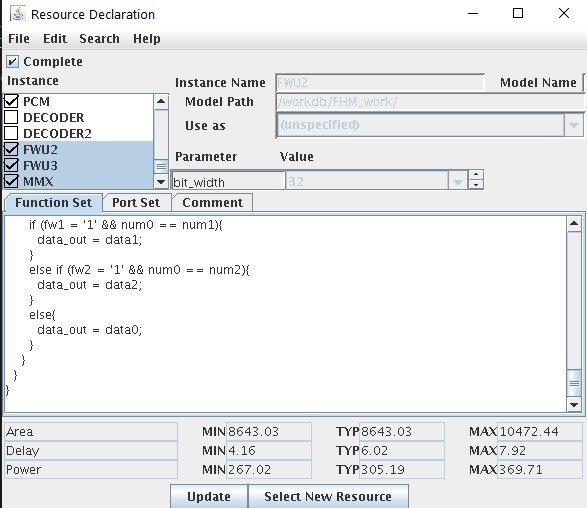
\includegraphics[width=0.8\textwidth]{src/images/image1.jpg}
	\caption{}
	\label{fig:fig1}
\end{figure}
\item Then, create a new instruction formats with two input and two output
registers. And create two different instructions which will use
existing and new resources respectively.
\begin{figure}[!htb]
	\centering
	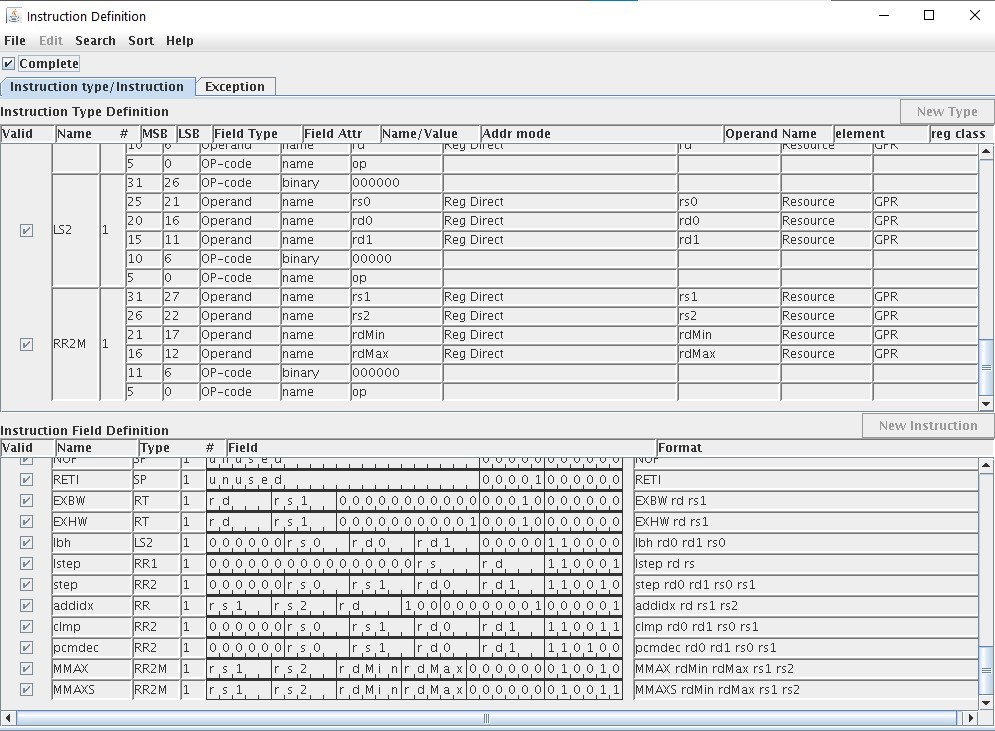
\includegraphics[width=0.8\textwidth]{src/images/image2.jpg}
	\caption{}
	\label{fig:fig2}
\end{figure}
\item The Micro-Op description for the instruction MMAXS, which will be
using the existing resources of ASIPmeister.
\begin{figure}[!htb]
	\centering
	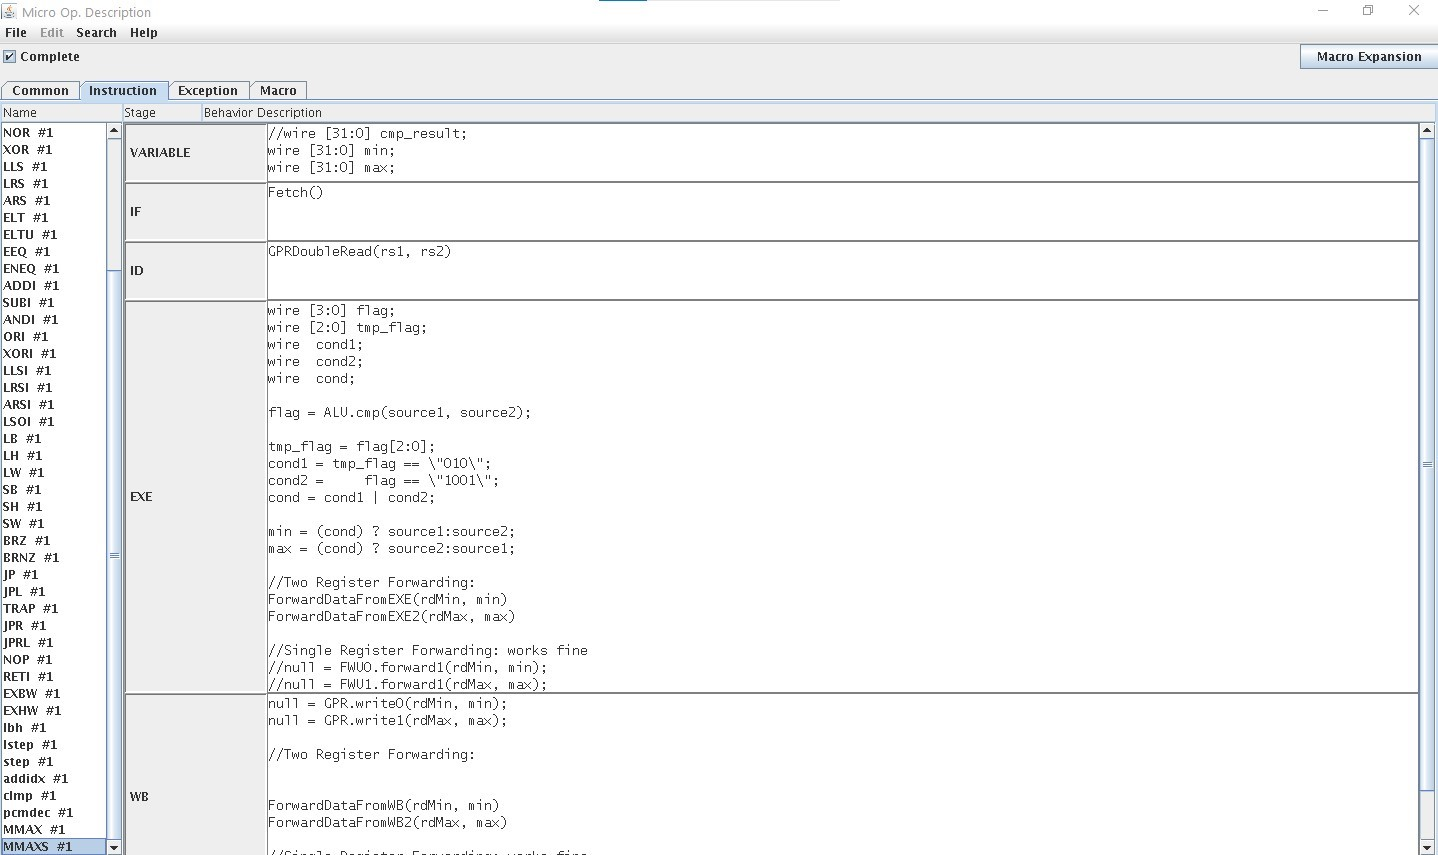
\includegraphics[width=0.8\textwidth]{src/images/image3.jpg}
	\caption{}
	\label{fig:fig3}
\end{figure}
\end{enumerate}
\subsubsection{USING NEW RESOURCES}
\begin{enumerate}[resume]
\item The Micro-Op description for the instruction \textbf{MMAX}, which will
be using the new resource \textbf{MMX} of ASIPmeister.
\begin{figure}[!htb]
	\centering
	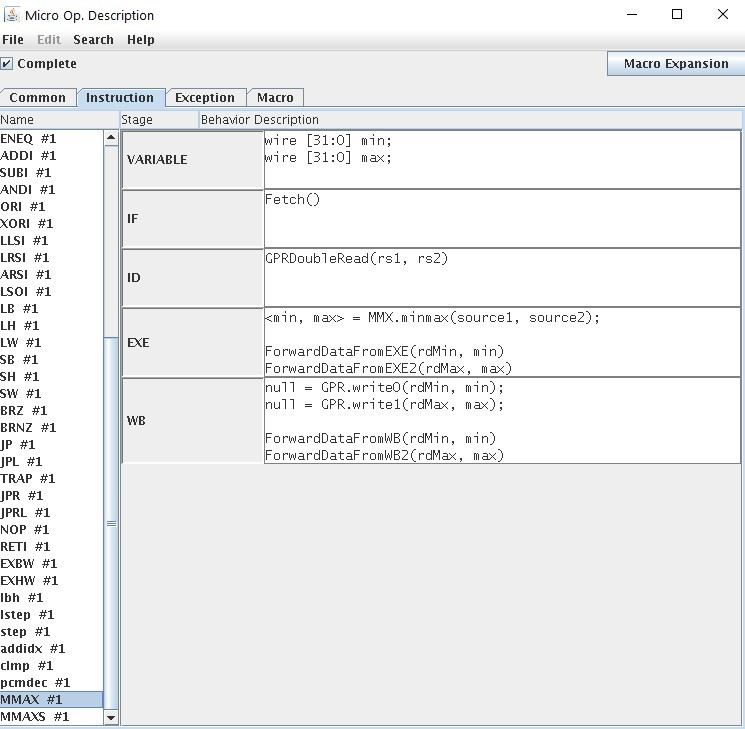
\includegraphics[width=0.8\textwidth]{src/images/image4.jpg}
	\caption{}
	\label{fig:fig4}
\end{figure}
\item C Definition may look like this.
\begin{figure}[!htb]
	\centering
	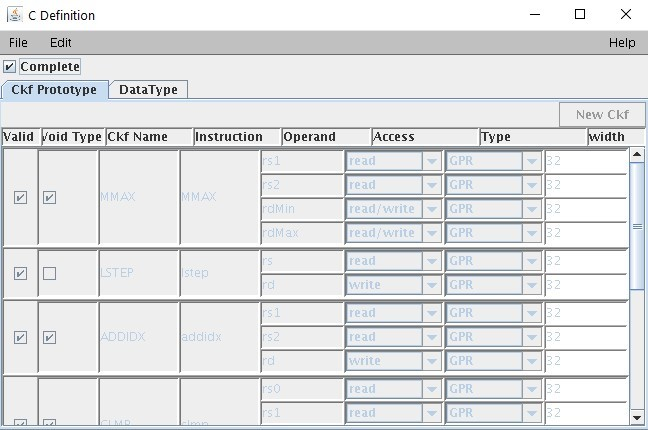
\includegraphics[width=0.8\textwidth]{src/images/image5.jpg}
	\caption{}
	\label{fig:fig5}
\end{figure}
\item Generate the required compiler and VHDL files. A
``\emph{\textbf{meister}}'' directory will be created in your ASIP
project directory i.e. in ``\emph{\textbf{brownie}}''
\item Create a ModelSim project in the relevant directory of the current
project, compile it and make it ready for the simulation.
\end{enumerate}
\subsection{USING INSTRUCTIONS}
\begin{enumerate}[resume]
\item Goto the ``Applications'' folder and create different applications to
test each.
\end{enumerate}
\subsubsection{ORIGINAL APPLICATION}
\begin{lstlisting}
sajjad@i80pc57:~/SS21/ASIPMeisterProjects/8/
brownie/Applications/ testMinMaxAPP:$ vim test.c
\end{lstlisting}
\begin{lstlisting}[language=C,caption={"test.c using original"},captionpos=t]
#define max(a, b) ( (a)>(b) ? (a):(b) )
#define min(a, b) ( (a)<(b) ? (a):(b))
unsigned int A[10] = { 32, 45, 0,0,0,0,0,0,0};
int main() {
	A[4]  = max(A[0], A[1]); // Maximum
	A[5]  = min(A[0], A[1]); // Minimum
	return 0;
}
\end{lstlisting}
\subsubsection{APPLICATION WITH MMAXS (Existing Resources)}
\begin{lstlisting}
sajjad@i80pc57:~/SS21/ASIPMeisterProjects/8/
brownie/Applications/ testMinMaxSW:$ vim test.c
\end{lstlisting}
\begin{lstlisting}[language=C,caption={"test.c using existing resources"},captionpos=t]
unsigned int A[10] = { 32, 45, 0,0,0,0,0,0,0};
int main() {
	__asm__ volatile (
	"mmaxs %[out1], %[out2], %[op1], %[op2]\n\t"
	: [out1] "=&r" (A[5]), [out2] "=&r" (A[4])
	: [op1] "r" (A[0]), [op2] "r" (A[1])
	);
	return 0;
}	
\end{lstlisting}
\subsubsection{APPLICATION WITH MMAX (New Resources)}
\begin{lstlisting}
sajjad@i80pc57:~/SS21/ASIPMeisterProjects/8/
brownie/Applications/ testMinMaxHW:$ vim test.c
\end{lstlisting}
\begin{lstlisting}[language=C,caption={"test.c using added resources"},captionpos=t]
unsigned int A[10] = { 32, 45, 0,0,0,0,0,0,0};
int main() {
	__asm__ volatile (
	"mmax %[out1], %[out2], %[op1], %[op2]\n\t"
	: [out1] "=&r" (A[5]), [out2] "=&r" (A[4])
	: [op1] "r" (A[0]), [op2] "r" (A[1])
	);
	
	return 0;
}
\end{lstlisting}
\subsubsection{MODELSIM SIMULATIONS}
\begin{enumerate}[resume]
\item ModelSim simulations produces following values:
\begin{lstlisting}
testMinMaxAPP
-----------------
# ** Failure: SUCCESSFUL: Simulation End.
#    Time: 2205 ns  Iteration: 0  Process: /test/dmem File: /home/sajjad/SS21/ASIPMeisterProjects/8/dlx_opt_performance_1/ModelSim/tb_browstd32.vhd
# Break in Process dmem at /home/sajjad/SS21/ASIPMeisterProjects/8/dlx_opt_performance_1/ModelSim/tb_browstd32.vhd line 603

testMinMaxSW 
-----------------
# ** Failure: SUCCESSFUL: Simulation End.
#    Time: 1195 ns  Iteration: 0  Process: /test/dmem File: /home/sajjad/SS21/ASIPMeisterProjects/8/dlx_opt_performance_1/ModelSim/tb_browstd32.vhd
# Break in Process dmem at /home/sajjad/SS21/ASIPMeisterProjects/8/dlx_opt_performance_1/ModelSim/tb_browstd32.vhd line 603

testMinMaxHW 
-----------------
# ** Failure: SUCCESSFUL: Simulation End.
#    Time: 1195 ns  Iteration: 0  Process: /test/dmem File: /home/sajjad/SS21/ASIPMeisterProjects/8/dlx_opt_performance_1/ModelSim/tb_browstd32.vhd
# Break in Process dmem at /home/sajjad/SS21/ASIPMeisterProjects/8/dlx_opt_performance_1/ModelSim/tb_browstd32.vhd line 603
\end{lstlisting}
\end{enumerate}